\setcounter{table}{0}   %从0开始编号，显示出来表会A1开始编号
\setcounter{figure}{0}
\setcounter{section}{0}
\setcounter{equation}{0}
%定义编号格式，在数字序号前加字符“A"
\renewcommand{\thetable}{A\arabic{table}}
\renewcommand{\thefigure}{A\arabic{figure}}
\renewcommand{\thesection}{A\arabic{section}}
\renewcommand{\theequation}{A\arabic{equation}}

% 附录内容：
% task的定义。 提供数据集的示例, LogAD数据集是如何生成的: 日志解析方法，滑动窗口 Template等等   实验的具体设置   各个client的loss曲线


\section{Conversation Template}
As shown in Figure \ref{fig:template}, we show two conversation templates (prompts) integrated with specific input parts (in \textcolor{red}{red}). These templates serve as structured input frameworks for guiding LLMs to generate desired outputs. By providing context and constraints through these prompts, LLMs can effectively process and respond to inputs in a targeted manner, enhancing the quality and relevance of generated outputs. This integration of prompts with input segments facilitates more precise and contextually appropriate responses from LLMs, contributing to improved performance and usability in various natural language processing tasks.
\begin{figure}[!ht]
    \centering
    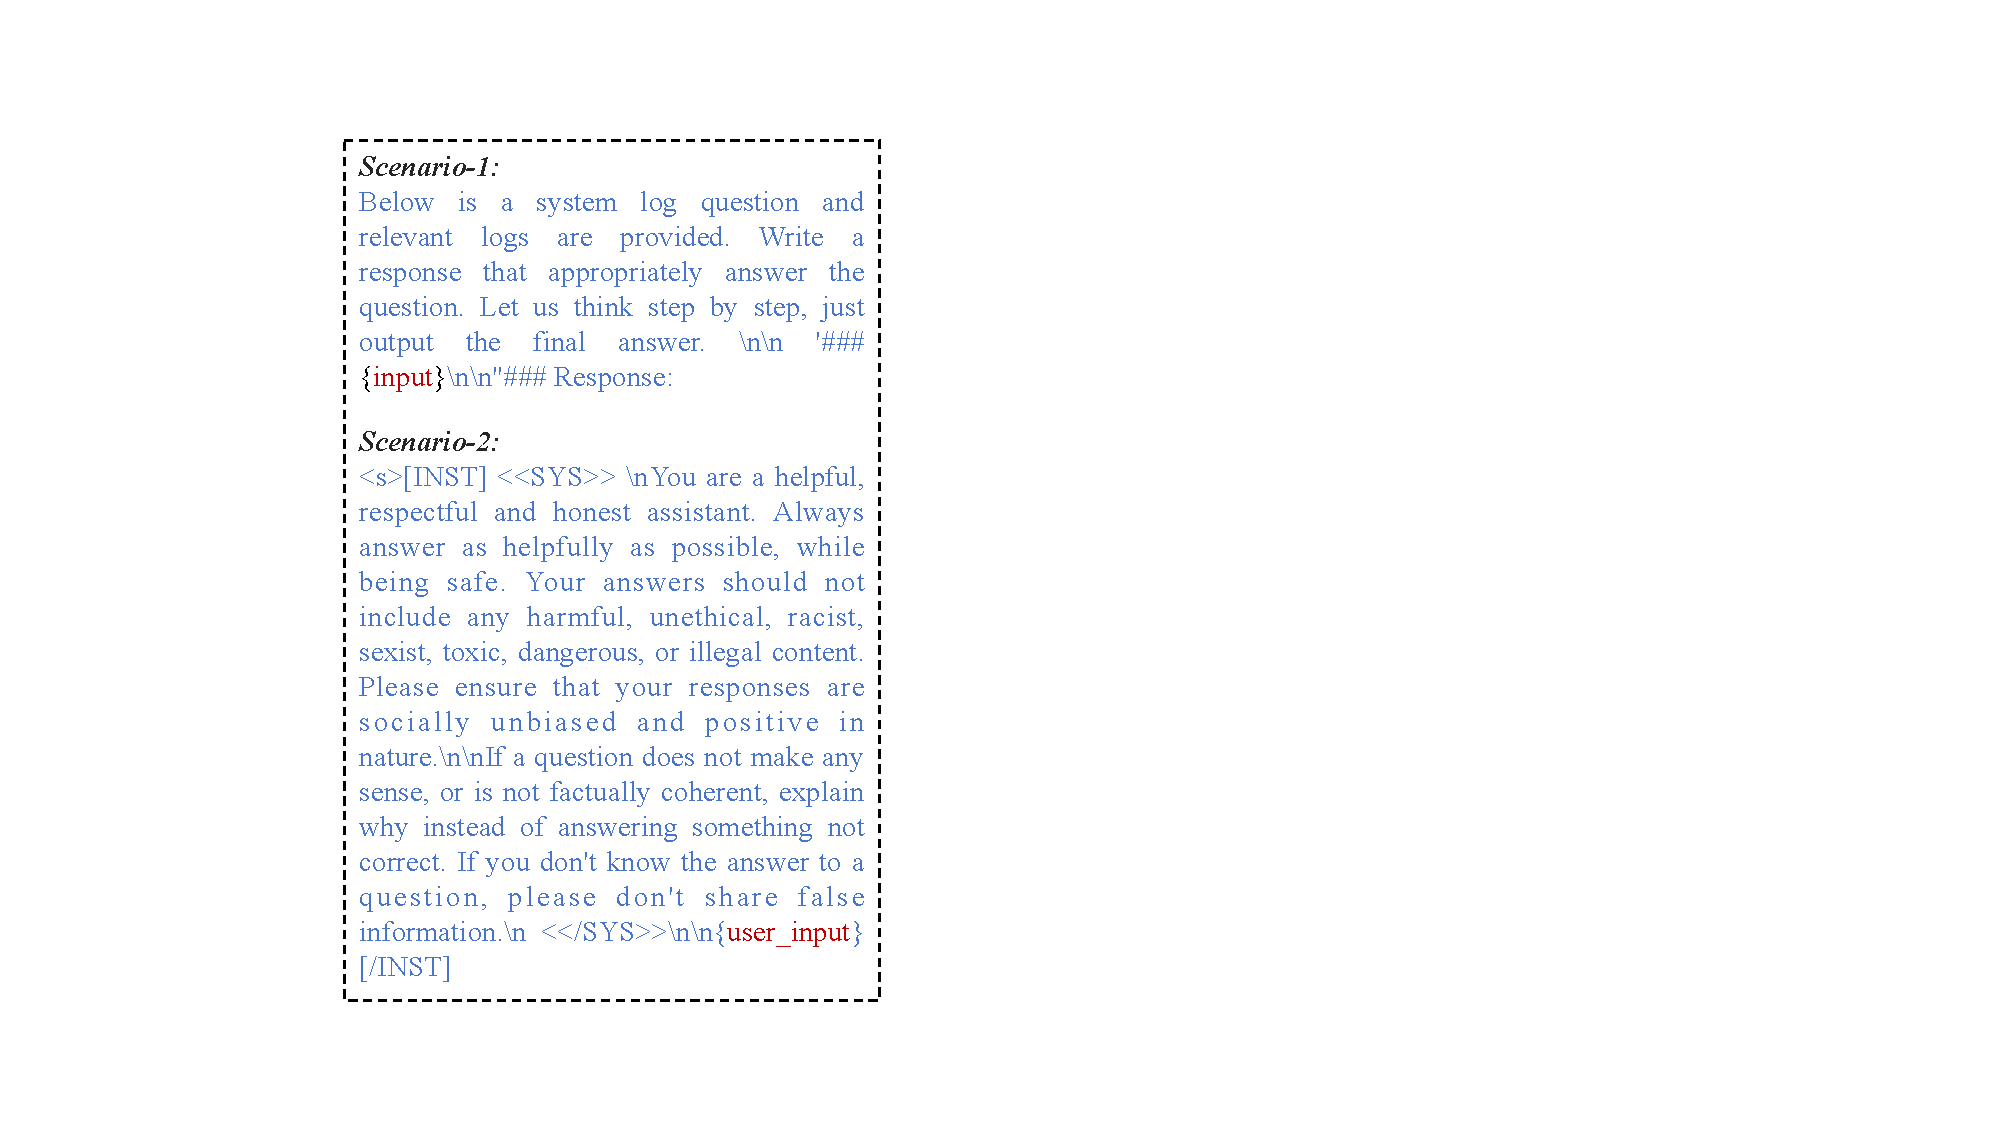
\includegraphics[scale=0.8]{figs/template.pdf}
    \caption{Conversation template with both log-based anomaly detection and medical diagnosis.}
    \label{fig:template}
\end{figure}
\section{Dataset Example}
Figure \ref{fig:data_sample} shows the format of the training data in both scenarios. The format is important for the training process. All training data is stored in JSON format, a popular data format. 
\begin{figure}[!ht]
    \centering
    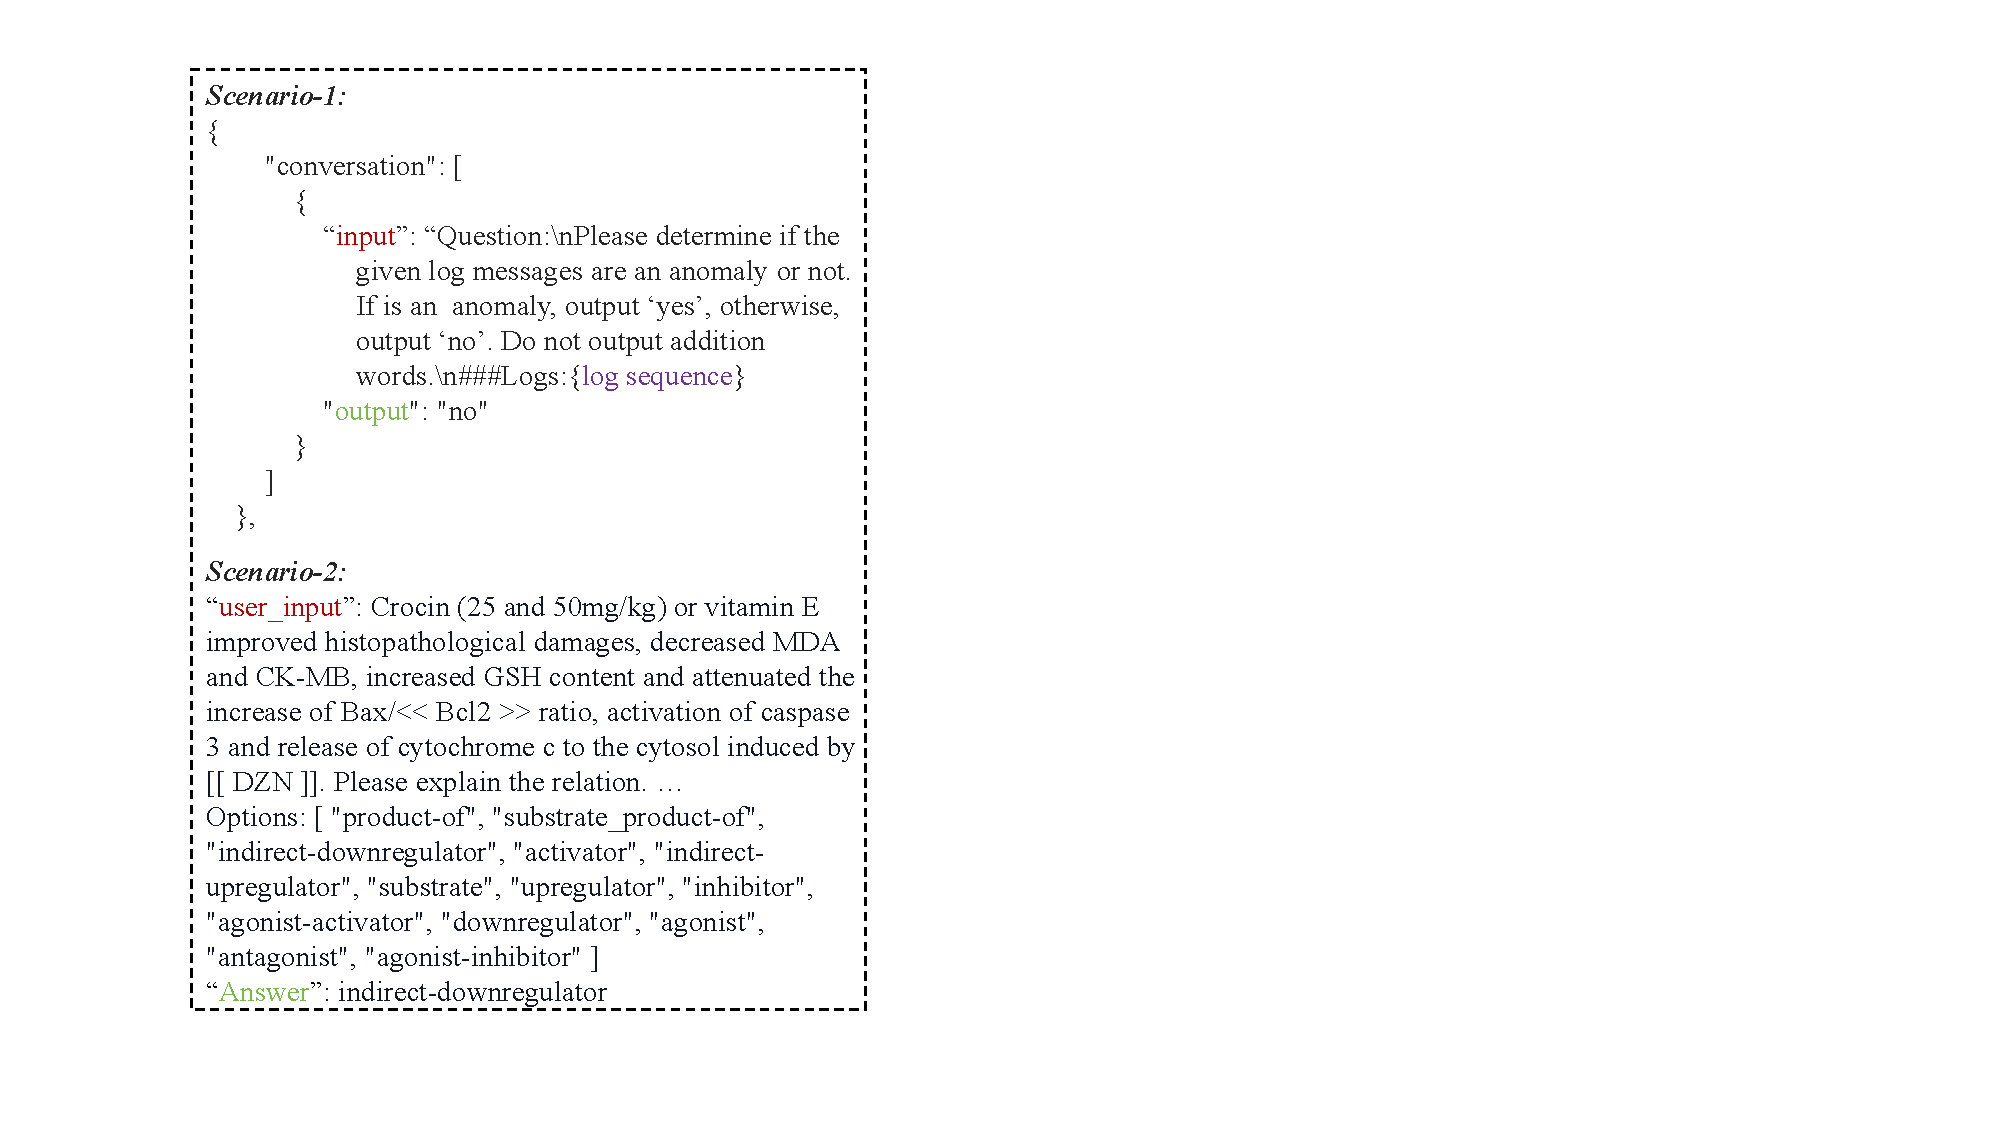
\includegraphics[scale=0.7]{figs/data_sample.pdf}
    \caption{Data example with both log-based anomaly detection and medical diagnosis.}
    \label{fig:data_sample}
\end{figure}

\section{Data prepossessing}
\begin{figure}[!ht]
    \centering
    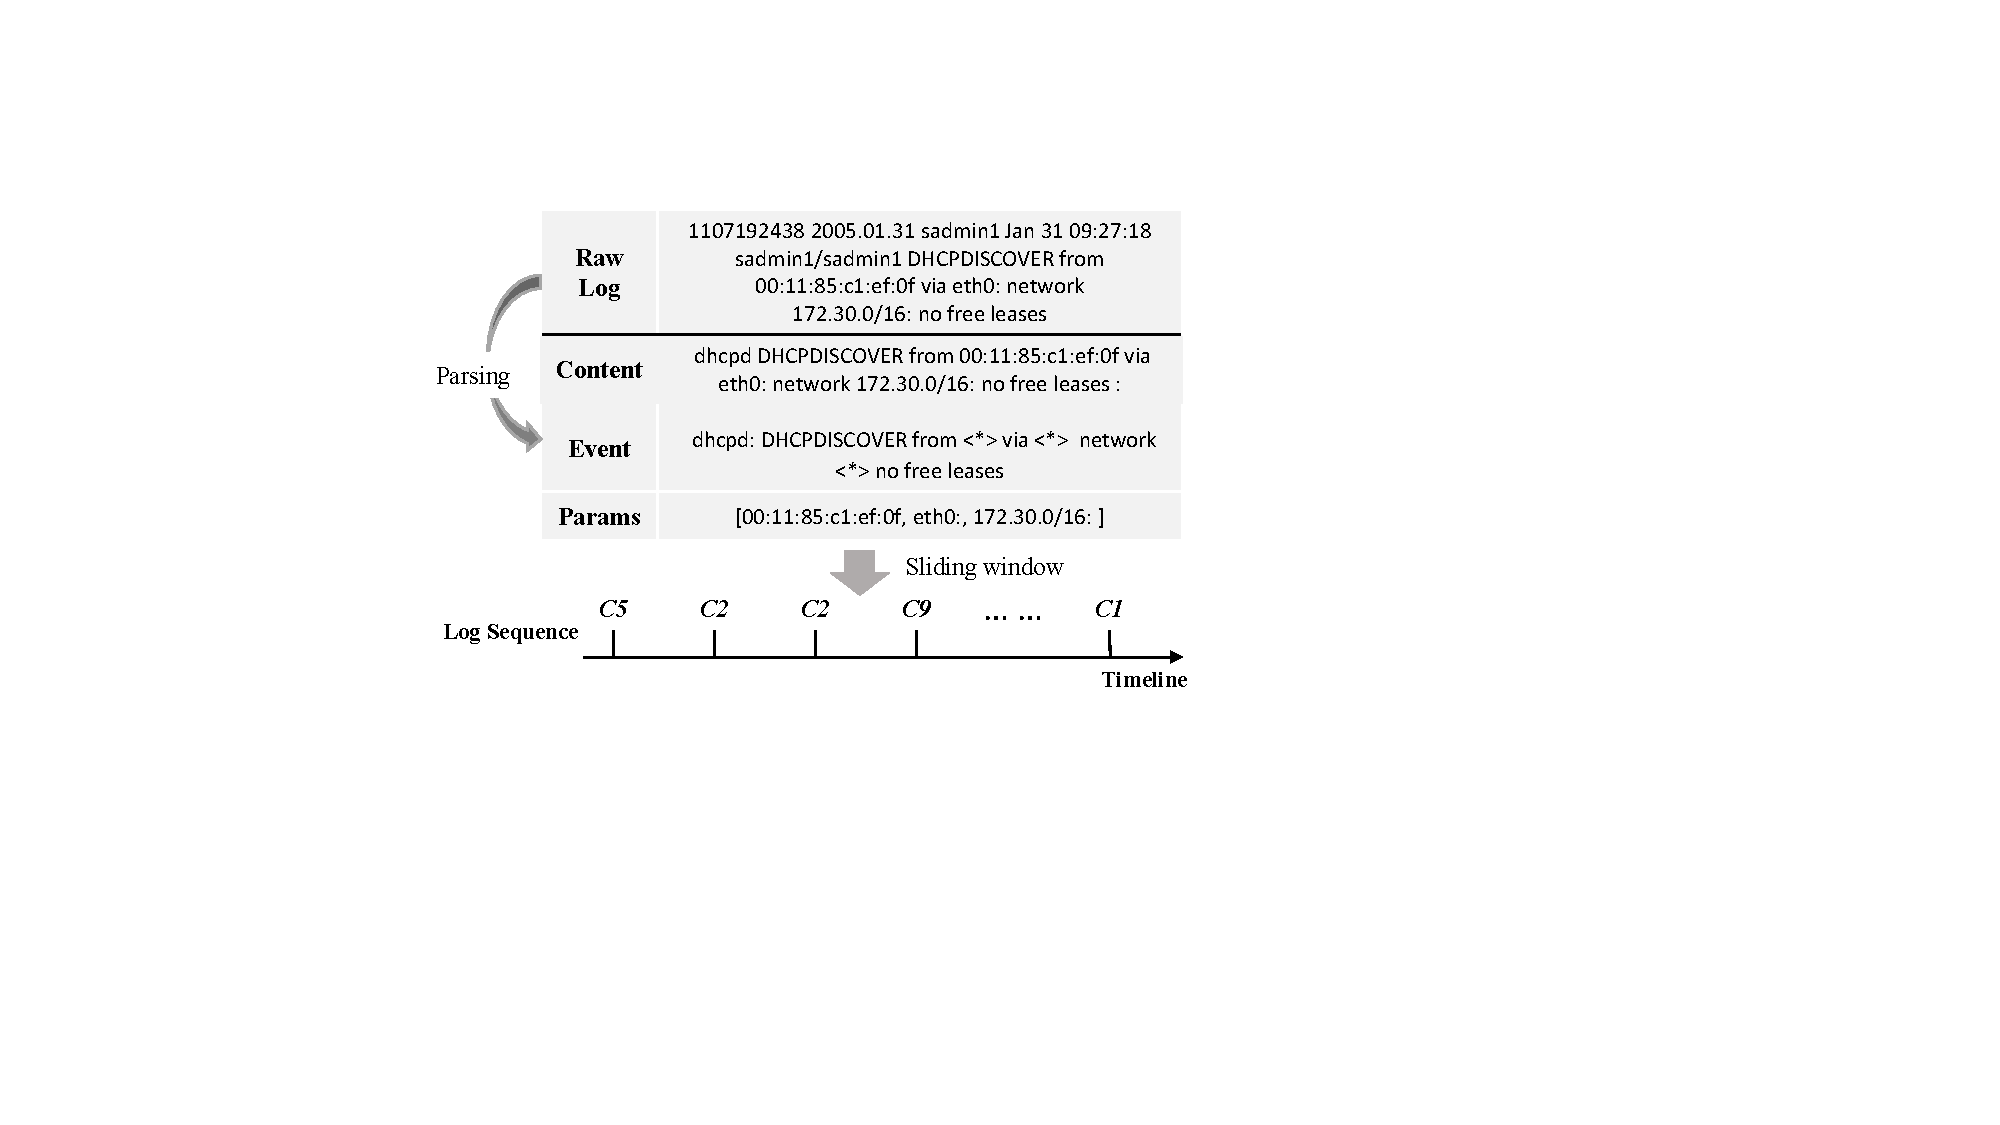
\includegraphics[scale=0.6]{figs/log_process.pdf}
    \caption{The illustration of log preprocessing.}
    \label{fig:log_process}
\end{figure}

Figure \ref{fig:log_process} is the illustration of preprocessing raw log messages. Log messages typically exhibit a semi-structured format, comprising two main components: a consistent part of the log event, and a variable part containing parameters. To prepare log data for anomaly detection model training, several preprocessing steps are necessary. Initially, both prefix and noise are eliminated through log filtering procedures to obtain the content part. Subsequently, automated log parsing techniques, such as Drain, are applied to extract both log events and parameters. Once parsed, the logs are organized into distinct groups using a fixed-size sliding window (the size default is 50), each comprising multiple log records. These groupings, designated as log sequences, serve as inputs for anomaly detection models and facilitate the identification of various patterns present in the log data. Note that based on existing work, the content part was selected to form the sequence to improve detection performance.

\section{Experiment Environment Details}
As shown in Table \ref{tab:system}, we present the experimental hardware environment and details of LLaMA2-7B. In particular, we used three homogenous devices, so 6 $\times$ V100s were included in total.

\begin{table}[!hb]
\centering
\caption{The evaluated system and LLM specifications. }
\label{tab:system}
\begin{tabular}{ll} 
\toprule
                           & \textbf{System Overview}  \\
                           \midrule
\textbf{CPU}               & 48-core Xeon(R) Gold 6126 CPU @ 2.60GHz       \\
\textbf{GPU}               & 2 $\times$ Tesla V100S       \\
\textbf{Memeory Capacity}  & 187GB DRAM                                    \\
\textbf{Operating System}  & CentOS 7.5.1804                               \\
\textbf{CUDA}              & 12.1                                          \\
\textbf{NVIDIA Driver}     & 530.30.02                                     \\
\textbf{ML framework}      & Pytorch 2.1.2                                 \\
\midrule
                           & \textbf{GPU Specification }                            \\
\midrule
\textbf{CUDA cores}        & 5120                                          \\
\textbf{Memeory Capacity}  & 32GB                                          \\
\textbf{Memeory Bandwidth} & 900GB/s                                       \\
\midrule
                           & \textbf{LLaMA2-7B }                                    \\
\midrule
\textbf{\#Tokens}          & 2.0T                                          \\
\textbf{\#Vocab}           & 32,000                                        \\
\textbf{Seq.Length}        & 4K                                            \\
\textbf{\#Layer}           & 32                                            \\
\bottomrule
\end{tabular}
\end{table}
